%%%%%%%%%%%%%%%%%%%%%%%%%%%%%%%%%%%%%%%%%
% Appendix
% 
% $Date$
% $Rev$:
% $Author$


\appendix
\renewcommand{\thesection}{\Alph{section}} \setcounter{section}{0}
\chapter*{Appendix}
\addcontentsline{toc}{chapter}{Appendix}
  \section{\KiekerMonitoringPart{} Configuration File}\label{sec:appdx:monitoringproperties}

This is the file \file{\monitoringPropertiesFile} from the binary release and 
constitutes \KiekerMonitoringPart{}'s default configuration.

\

\setXMLListing
\lstinputlisting[caption=\monitoringPropertiesFile]{../../META-INF/kieker.monitoring.properties}

\newpage


  \section{Additional Source Code Listings}
    \subsection{MyNamedPipeManager and MyPipe}
      \setJavaCodeListing
      \lstinputlisting[caption=MyNamedPipeManager.java]{\customComponentsBookstoreApplicationDir/src/bookstoreApplication/MyNamedPipeManager.java}

      \setJavaCodeListing
      \lstinputlisting[caption=MyPipe.java]{\customComponentsBookstoreApplicationDir/src/bookstoreApplication/MyPipe.java}

\newpage
  \section{Example File System Monitoring Logs}

	\subsection{Chapter \ref{chap:example}}
		The following listing shows the produced log during a run of the Bookstore Application with the manual monitoring probes.
		\setTextListing
\lstinputlisting[caption=Execution of the manually instrumented Bookstore application (Section~\ref{sec:example:monitoring})]
{ch2-quickstart-example/kieker-20120402-163314855-UTC-myHost-KIEKER-SINGLETON-monitoring.stdout}
		The second listing is the log during the analysis of the produced data. It can be seen that some of the calls are accepted and some others refused.
		\setTextListing
\lstinputlisting[caption=Execution of the example analysis (Section~\ref{sec:example:analysis})]
{ch2-quickstart-example/kieker-20130910-120352847-UTC-myHost-KIEKER-SINGLETON-analysis.stdout}
	
	\subsection{Chapter \ref{chap:aspectJ}}
	    The following listing shows the produced log during a run of the Bookstore Application, weaved with the necessary code at runtime as shown in Section \ref{sec:aspectJ:fullweaving}.
		\setTextListing
\begin{lstlisting}[caption=Execution of the Bookstore with AspectJ trace instrumentation (Section~\ref{sec:traceAnalysis:instr:AspectJ})]
Bookstore.main: Starting request 0
10.04.2012 13:03:51 kieker.monitoring.core.configuration.ConfigurationFactory createSingletonConfiguration
INFO: Loading properties from properties file in classpath: 'META-INF/kieker.monitoring.properties'
10.04.2012 13:03:51 kieker.monitoring.core.controller.MonitoringController createInstance
INFO: Current State of kieker.monitoring (1.5) Status: 'enabled'
        Name: 'KIEKER'; Hostname: 'pc-vanhoorn'; experimentID: '1'
JMXController: JMX disabled
RegistryController: 0 strings registered.
TimeSource: 'kieker.monitoring.timer.SystemNanoTimer'
        Time in nanoseconds (with nanoseconds precision) since Thu Jan 01 01:00:00 CET 1970'
WriterController:
        Number of Inserts: '0'
        Automatic assignment of logging timestamps: 'true'
Writer: 'kieker.monitoring.writer.filesystem.AsyncFsWriter'
        Configuration:
                kieker.monitoring.writer.filesystem.AsyncFsWriter.QueueFullBehavior='0'
                kieker.monitoring.writer.filesystem.AsyncFsWriter.flush='true'
                kieker.monitoring.writer.filesystem.AsyncFsWriter.QueueSize='10000'
                kieker.monitoring.writer.filesystem.AsyncFsWriter.customStoragePath='.'
                kieker.monitoring.writer.filesystem.AsyncFsWriter.MaxShutdownDelay='-1'
                kieker.monitoring.writer.filesystem.AsyncFsWriter.storeInJavaIoTmpdir='true'
                kieker.monitoring.writer.filesystem.AsyncFsWriter.maxEntriesInFile='25000'
        Records lost: 0
        Writer Threads (1): 
                Finished: 'false'; Writing to Directory: '/tmp/kieker-20110428-142829399-UTC-Kaapstad-KIEKER'
Sampling Controller: Periodic Sensor available: Current Poolsize: '0'; Scheduled Tasks: '0'

10.04.2012 13:03:51 kieker.monitoring.core.registry.ControlFlowRegistry <clinit>
INFO: First threadId will be 7752665283541598209
10.04.2012 13:03:51 kieker.monitoring.core.controller.MonitoringController$\$$1 run
INFO: ShutdownHook notifies controller to initiate shutdown
10.04.2012 13:03:51 kieker.monitoring.core.controller.MonitoringController cleanup
INFO: Shutting down Monitoring Controller (KIEKER)
10.04.2012 13:03:51 kieker.monitoring.writer.AbstractAsyncWriter terminate
INFO: Shutting down writers.
\end{lstlisting}



	
\newpage
  \section{Ant Scripts}
    \subsection{Chapter \ref{chap:example}}
      Following listings show the necessary \file{build.xml} and \file{build.properties} to compile and execute the manual instrumentated Bookstore Application shown in Chapter~\ref{chap:example}.
      \setXMLListing
      \lstinputlisting[caption=build.xml]{\manualInstrumentedBookstoreApplicationDir/build.xml}
      \lstinputlisting[caption=build.properties]{\manualInstrumentedBookstoreApplicationDir/build.properties}
      In order to run the analysis of the application, it is still necessary to supply the program with the path to the output directory of the monitoring. This is done via the parameter "analysis.directory", e.g.:
      \setBashListing
      \begin{lstlisting}[caption=Command to compile and run the instrumented Bookstore via ant]
#\lstshellprompt{}# ant run-analysis -Danalysis.directory /tmp/kieker-20120402-163314855-UTC-myHost-KIEKER-SINGLETON
\end{lstlisting}%-KIEKER


    \subsection{Chapter \ref{chap:componentsMonitoring} and \ref{chap:componentsAnalysis}}
      Following listings show the necessary \file{build.xml} and \file{build.properties} to compile and execute the manually instrumentated Bookstore Application with the own components shown in Chapter~\ref{chap:componentsMonitoring} and \ref{chap:componentsAnalysis}.
      \setXMLListing
      \lstinputlisting[caption=build.xml]{\customComponentsBookstoreApplicationDir/build.xml}
      \lstinputlisting[caption=build.properties]{\customComponentsBookstoreApplicationDir/build.properties}

    \subsection{Chapter \ref{chap:aspectJ}}
      Following listings show the necessary \file{build.xml} and \file{build.properties} to compile and execute the Bookstore Application instrumentated with AspectJ shown in Chapter~\ref{chap:aspectJ}.
      \setXMLListing
      \lstinputlisting[caption=build.xml]{\aspectJBookstoreApplicationDir/build.xml}
      \lstinputlisting[caption=build.properties]{\aspectJBookstoreApplicationDir/build.properties}     

\newpage
  \section{Example Graphs and Diagrams}
    \begin{figure}[H]\centering
	\subfigure[]{\label{fig:appendix:aggregatedAllocationCallTree}%
	\includegraphics[width=0.33\textwidth]{images/aggregatedAllocationCallTree}%
	}%
	\subfigure[]{\label{fig:appendix:aggregatedAssemblyCallTree}%
	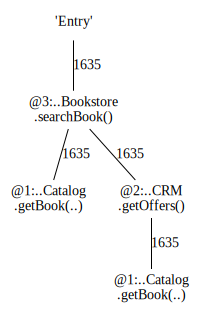
\includegraphics[width=0.33\textwidth]{images/aggregatedAssemblyCallTree}%
	}%
	\subfigure[]{\label{fig:appendix:callTree}%
	\includegraphics[width=0.33\textwidth]{images/callTree}%
	}%
	\caption{Aggregated Allocation Call Tree~\subref{fig:appendix:aggregatedAllocationCallTree}, Aggregated Assembly Call Tree~\subref{fig:appendix:aggregatedAssemblyCallTree} and Call Tree~\subref{fig:appendix:callTree}}
	\end{figure}
	
    \begin{figure}[H]\centering
	\subfigure[]{\label{fig:appendix:allocationComponentDependencyGraph}%
	\includegraphics[width=0.8\textwidth]{images/allocationComponentDependencyGraph}
	}\\
	\subfigure[]{\label{fig:appendix:assemblyComponentDependencyGraph}%
	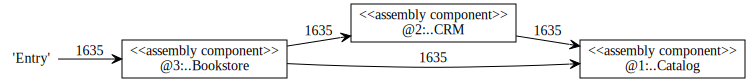
\includegraphics[width=0.8\textwidth]{images/assemblyComponentDependencyGraph}
	}%
	\caption{Allocation Component Dependency Graph~\subref{fig:appendix:allocationComponentDependencyGraph} and Assembly Component Dependency Graph~\subref{fig:appendix:assemblyComponentDependencyGraph}}
	\end{figure}
	
	\begin{figure}[H]\centering
	\subfigure[]{\label{fig:appendix:allocationOperationDependencyGraph}%
	\includegraphics[width=0.8\textwidth]{images/allocationOperationDependencyGraph}
	}\\
	\subfigure[]{\label{fig:appendix:assemblyOperationDependencyGraph}%
	\includegraphics[width=0.8\textwidth]{images/assemblyOperationDependencyGraph}
	}%
	\caption{Allocation Operation Dependency Graph~\subref{fig:appendix:allocationOperationDependencyGraph} and Allocation Operation Dependency Graph~\subref{fig:appendix:assemblyOperationDependencyGraph}}
	\end{figure}
	
	\begin{figure}[H]\centering
	\subfigure[]{\label{fig:appendix:allocationSequenceDiagram}
	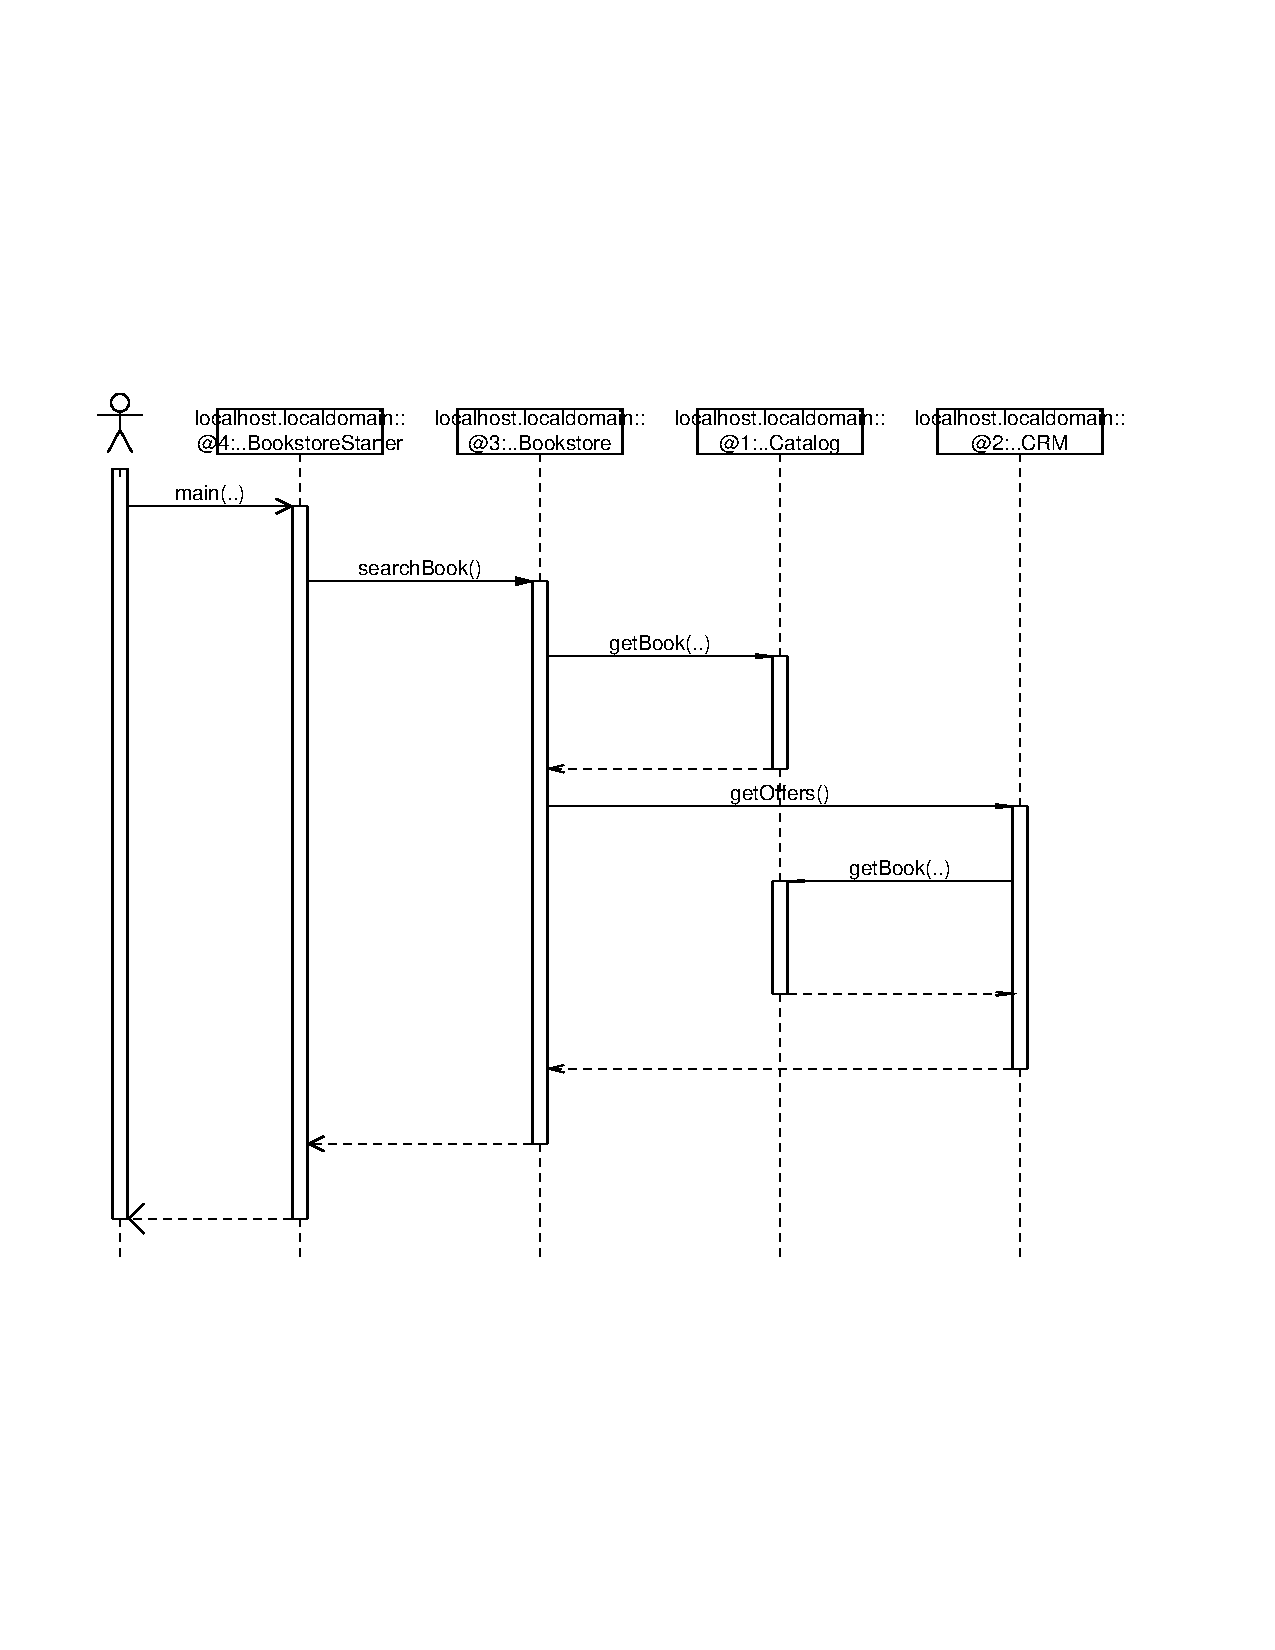
\includegraphics[width=0.4\textwidth]{images/allocationSequenceDiagram}
	}
	\subfigure[]{\label{fig:appendix:assemblySequenceDiagram}
	\includegraphics[width=0.4\textwidth]{images/assemblySequenceDiagram}
	}
	\caption{Allocation Sequence Diagram~\subref{fig:appendix:allocationSequenceDiagram} and Assembly Sequence Diagram~\subref{fig:appendix:assemblySequenceDiagram}}
	\end{figure}
	
	\begin{figure}[H]
		\centering
		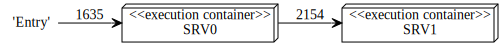
\includegraphics[width=0.5\textwidth]{images/containerDependencyGraph}
		\caption{Container Dependency Graph}
	\end{figure}
  
  
\newpage
  \section{Libraries}
    The following table shows all libraries which are used by \Kieker\ and explains them briefly.
    \begin{center}
\begin{longtable}{|p{0.4\textwidth}|p{0.5\textwidth}|}
\hline 
Filename & Description\\
\hline
\hline 
aspectjrt-1.6.11.jar & This jar-file contains the runtime library for AspectJ programs.\\
\hline 
aspectjtools-1.6.11.jar & This package contains the tools (the AspectJ Compiler and Browser) for AspectJ.\\
\hline 
aspectjweaver-1.6.11.jar & This jar contains the weaver-agent for the aspect-oriented-extension for Java named AspectJ.\\
\hline 
commons-cli-1.2.jar & Apache Commons CLI provides a simple API for working with the command line arguments and options.\\
\hline 
commons-logging-1.1.1.jar & Apache Commons Logging is a thin adapter allowing configurable bridging to other, well known logging systems.\\
\hline 
cxf-api-2.2.10.jar & Apache CXF is an open source services framework.  \\
\hline 
cxf-common-utilities-2.2.10.jar & This package contains different classes for Apache CXF.\\
\hline 
cxf-rt-bindings-soap-2.2.10.jar & This package contains necessary files to use Apache CXF as well with the Simple Object Access Protocol (SOAP).\\
\hline 
cxf-rt-core-2.2.10.jar & This library contains the Apache CXF Runtime Core. \\
\hline 
derby.jar & Apache Derby is a lightweight database written in Java which can also be used as an embedded database. This library contains the necessary drivers for the database as well as the database management system itself.\\
\hline 
jms-1.1.jar & Java Message Service is an API to send and receive messages within a client and to control so called Message Oriented Middleware (MOM).\\
\hline 
jndi-1.2.1.jar & The Java Naming and Directory Interface is an API which provides methods for multiple naming and directory services. It can be used for example to register disposed files in a network and to allow other part of a Java program to use them for RMI calls.\\
\hline 
junit-4.5.jar & This jar-file contains the necessary classes for the JUnit-tests, which can be used to test automatically Java classes.\\
\hline 
log4j-1.2.15.jar & Apache log4j is a framework for the logging of messages, errors and exceptions in Java applications.\\
\hline 
servlet-api.jar & The Java Servlet API supplies protocols to let applications respond for example to HTTP requests.\\
\hline 
sigar-1.6.3.jar & Hyperic SIGAR (System Information Gatherer) provides a Java API to system inventory and monitoring data (Memory, CPU etc.). In addition to the Jar file, it is required to add corresponding platform-specific native libraries to the classpath, which can be downloaded from~\cite{HypericSigarWebsite}. Kieker's \dir{lib/} folder already includes such libraries for Linux/Windows for the x86~architecture (\file{libsigar-x86-linux.so} and \file{sigar-x86-winnt.[dll|lib]}.\\
\hline 
spring.jar & The spring framework delivers different methods and classes to make the handling with Java/Java EE easier.\\
\hline 
spring-web.jar & This library contains the web application context, multipart resolver, Struts support, JSF support and web utilities for the spring framework.\\
\hline 
\end{longtable}
\label{tabular:libraries}
\end{center}


% \chapter{Troubleshooting}
